\documentclass[12pt,12pt,a4paper,oneside,bibliography=totoc]{scrbook}

% Template based on https://github.com/jgm/pandoc-templates/blob/master/default.latex

  \usepackage{lmodern}

  \usepackage[onehalfspacing]{setspace}

\usepackage{amssymb,amsmath}
\usepackage{ifxetex,ifluatex}
\usepackage{fixltx2e} % provides \textsubscript

% Code Listings

\usepackage{listings}
\usepackage{color}

\definecolor{mygreen}{rgb}{0,0.6,0}
\definecolor{mygray}{rgb}{0.5,0.5,0.5}
\definecolor{mymauve}{rgb}{0.58,0,0.82}

\lstset{ %
  backgroundcolor=\color{white},   % choose the background color; you must add \usepackage{color} or \usepackage{xcolor}
  basicstyle=\footnotesize,        % the size of the fonts that are used for the code
  breakatwhitespace=false,         % sets if automatic breaks should only happen at whitespace
  breaklines=true,                 % sets automatic line breaking
  captionpos=b,                    % sets the caption-position to bottom
  commentstyle=\color{mygreen},    % comment style
  deletekeywords={...},            % if you want to delete keywords from the given language
  escapeinside={\%*}{*)},          % if you want to add LaTeX within your code
  extendedchars=true,              % lets you use non-ASCII characters; for 8-bits encodings only, does not work with UTF-8
  frame=single,                    % adds a frame around the code
  keepspaces=true,                 % keeps spaces in text, useful for keeping indentation of code (possibly needs columns=flexible)
  keywordstyle=\color{blue},       % keyword style
  language=Octave,                 % the language of the code
  morekeywords={*,...},            % if you want to add more keywords to the set
  numbers=left,                    % where to put the line-numbers; possible values are (none, left, right)
  numbersep=5pt,                   % how far the line-numbers are from the code
  numberstyle=\tiny\color{mygray}, % the style that is used for the line-numbers
  rulecolor=\color{black},         % if not set, the frame-color may be changed on line-breaks within not-black text (e.g. comments (green here))
  showspaces=false,                % show spaces everywhere adding particular underscores; it overrides 'showstringspaces'
  showstringspaces=false,          % underline spaces within strings only
  showtabs=false,                  % show tabs within strings adding particular underscores
  stepnumber=2,                    % the step between two line-numbers. If it's 1, each line will be numbered
  stringstyle=\color{mymauve},     % string literal style
  tabsize=2,                       % sets default tabsize to 2 spaces
  title=\lstname                   % show the filename of files included with \lstinputlisting; also try caption instead of title
}

% Tables
\usepackage{longtable,booktabs}

\usepackage{graphicx}
% Redefine \includegraphics so that, unless explicit options are
% given, the image width will not exceed the width or the height of the page.
% Images get their normal width if they fit onto the page, but
% are scaled down if they would overflow the margins.
\makeatletter
\def\ScaleWidthIfNeeded{%
 \ifdim\Gin@nat@width>\linewidth
    \linewidth
  \else
    \Gin@nat@width
  \fi
}
\def\ScaleHeightIfNeeded{%
  \ifdim\Gin@nat@height>0.9\textheight
    0.9\textheight
  \else
    \Gin@nat@width
  \fi
}
\makeatother

\setkeys{Gin}{width=\ScaleWidthIfNeeded,height=\ScaleHeightIfNeeded,keepaspectratio}%

% Margins of chapter heading
  \renewcommand*{\chapterheadstartvskip}{\vspace*{-1cm}}
  \renewcommand*{\chapterheadendvskip}{\vspace{1cm}}

\usepackage[T1]{fontenc}
\usepackage[utf8]{inputenc}

% Package to set page headers and footers
  \usepackage[automark,headsepline]{scrlayer-scrpage}
      \clearpairofpagestyles
      \cfoot[\pagemark]{\pagemark}
      \lehead{\headmark}
      \rohead{\headmark}
      \pagestyle{scrheadings}
  





  \usepackage[left=3cm,right=2.5cm,top=3.5cm,bottom=3cm,headsep=1.5cm]{geometry}


  \usepackage[backend=biber,style=alphabetic]{biblatex}
      \addbibresource{library.bib}
  



\usepackage[unicode=true]{hyperref}

\hypersetup{breaklinks=true,
            pdfauthor={Mike Wazowski},
            pdftitle={The Title of my Worldshaking Masterthesis},
            colorlinks=true,
            citecolor=blue,
            urlcolor=blue,
            linkcolor=magenta,
            pdfborder={0 0 0}}

\urlstyle{same}  % don't use monospace font for urls



\setlength{\parindent}{0pt}
\setlength{\parskip}{6pt plus 2pt minus 1pt}
\setlength{\emergencystretch}{3em}  % prevent overfull lines

  \setcounter{secnumdepth}{5}


  \usepackage{lipsum}
  \usepackage{tocbibind}
  \usepackage{tocloft}
  \renewcommand{\contentsname}{Table of Contents}
  \renewcommand{\listfigurename}{Figures}
  \renewcommand{\listtablename}{Tables}

\begin{document}

\frontmatter

  \begin{titlepage}
\begin{singlespace}

\pagenumbering{Alph}

% Ausgleich wegen Seitenrändern
\setlength{\hoffset}{-5mm} 
\setlength{\voffset}{-15mm}

\begin{center}

% Logo
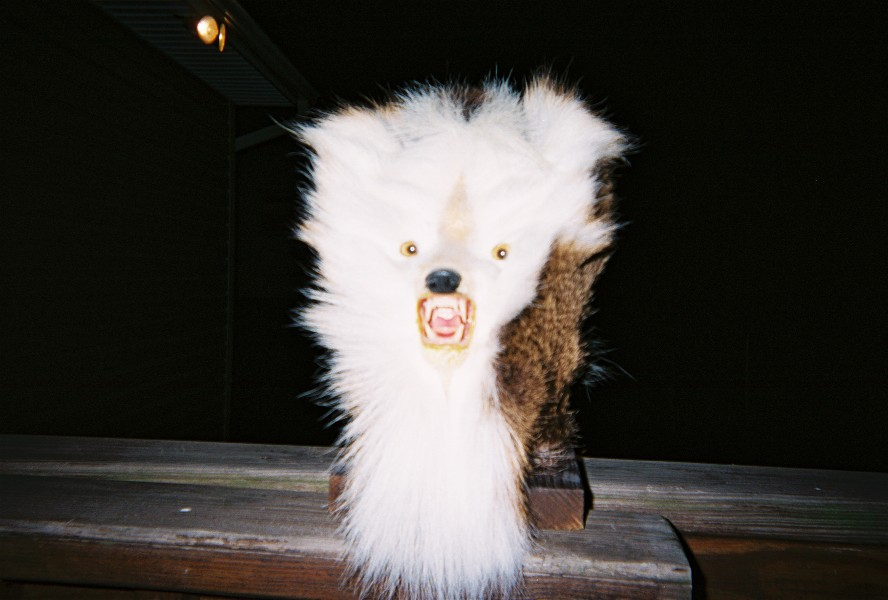
\includegraphics[width=6cm]{images/monster.jpg}\\

\vspace{1.5cm}
\LARGE
\textbf{The Title of my Worldshaking Masterthesis}\\

\vspace{1.5cm}

\large
\textbf{MASTERARBEIT}\\
\vspace{1.5cm}

\large
\textsc{
Monsters University\\
School of Scaring}\\

\vspace{1.5cm}

\textsc{Aufgabensteller: Prof. Dr. Tawny Van der Slime}\\
\smallskip
\textsc{Zweitkorrektur: Prof. Dr. Seecrus Jadeus}\\
\smallskip
\textsc{Betreuer: Timothy Rastrussen}\\


\vspace{1cm}
\textsc{Vorgelegt von\\
Mike Wazowski\\
Matrikelnummer: 4475204e657264203a29}\\

\vspace{1cm}
\textsc{Abgabe: \today}\\ %%Datum der Abgabe - am besten selbst reinschreiben.}

\end{center}

\clearpage
\setlength{\hoffset}{0mm}
\end{singlespace}
\end{titlepage}

  \chapter*{Eigenständigkeitserklärung}

\thispagestyle{empty}

\vspace{2cm}

\parbox{5cm}{\centering\hrule\medskip Familienname, Vorname}
\vspace{3cm}
\hfill
\parbox{5cm}{\centering\hrule\medskip Ort, Datum}

\vspace{-1cm}

\parbox{5cm}{\centering\hrule\medskip Geburtsdatum}
\vspace{3cm}
\hfill
\parbox{5cm}{\centering\hrule\medskip Studiengruppe / WS/SS}



\centering{\LARGE\textbf{Erklärung}}

\centering{Gemäß \S 40 Abs. 1 i. V. m. \S 31 Abs. 7 RaPO}

\vspace{.5cm}

\flushleft

Hiermit erkläre ich, dass ich die Masterarbeit selbständig verfasst, noch nicht anderweitig
für Prüfungszwecke vorgelegt, keine anderen als die angegebenen Quellen oder Hilfsmittel
benützt sowie wörtliche und sinngemäße Zitate als solche gekennzeichnet habe.

\vspace{20mm}
\begin{flushright}
.................................................

\textit{Unterschrift}

\end{flushright}

												
  \chapter{Abstract}

\pagenumbering{roman}
\setcounter{page}{1}

Bacon ipsum dolor amet rump pastrami beef ribs, boudin tri-tip jerky meatball ground round corned beef chicken picanha biltong shoulder. Corned beef meatball jerky t-bone chicken. Pork chuck tenderloin, brisket biltong turducken pork loin kevin andouille bacon cupim shoulder pancetta ribeye tongue. Beef ribs landjaeger picanha, rump chicken tri-tip brisket drumstick t-bone turkey. Frankfurter landjaeger ground round, beef pork chop bacon beef ribs kevin.

Shank landjaeger short ribs, pig swine meatloaf ground round corned beef hamburger. Cow fatback meatball short loin kevin tri-tip pig tail shoulder pork chop. Ball tip flank kevin ham meatball cow tail bacon. T-bone porchetta spare ribs, pancetta meatball bresaola bacon swine rump cupim. Andouille turducken bresaola, meatball pancetta picanha tenderloin hamburger corned beef swine pig salami ham shankle. Flank cow landjaeger ribeye pancetta corned beef bresaola sausage ground round spare ribs andouille filet mignon tail.

Doner jerky fatback pork chop leberkas corned beef pancetta tail tenderloin cupim. Sirloin jowl swine ribeye, filet mignon flank salami short ribs. Pork loin ribeye shank t-bone. Short loin corned beef short ribs turducken beef drumstick ball tip alcatra tongue porchetta chuck leberkas jerky picanha shankle. Filet mignon bresaola bacon pork chop pancetta. Turkey ham hock tri-tip ribeye, flank swine landjaeger. Beef turkey shankle shoulder ribeye pig, bacon pastrami spare ribs flank doner pork picanha turducken pork chop.

Pork loin doner pork belly, t-bone picanha ground round landjaeger biltong beef venison pork chop salami porchetta ham. Corned beef chicken bacon pastrami brisket. Jowl strip steak landjaeger filet mignon porchetta, corned beef jerky fatback leberkas alcatra t-bone venison. Porchetta short loin boudin jowl ham pig flank t-bone.

Strip steak chicken kevin boudin sirloin, doner jerky tail. Andouille rump pig swine tail brisket tongue ham hock flank pancetta porchetta. Sausage bacon picanha cupim. Spare ribs beef salami hamburger shoulder, pancetta ball tip bacon turducken. Tri-tip brisket pork loin, beef tail cupim corned beef.
  \chapter{Acknowledgements}

\lipsum[1]

\clearpage

  \hypersetup{linkcolor=black}
  \setcounter{tocdepth}{2}
  \newgeometry{left=3cm,right=2.5cm, top=1.5cm, bottom=3cm}
    \tableofcontents
    \pagestyle{plain}
    \cleardoublepage

  \newgeometry{left=3cm,right=2.5cm, top=1.5cm, bottom=3cm}
    \listoftables
  \restoregeometry
  \clearpage

  \newgeometry{left=3cm,right=2.5cm, top=1.5cm, bottom=3cm}
    \listoffigures
  \restoregeometry
  \clearpage

      \clearpairofpagestyles
      \cfoot[\pagemark]{\pagemark}
      \lehead{\headmark}
      \rohead{\headmark}
      \pagestyle{scrheadings}
  
\mainmatter

\hyperdef{}{intro}{\chapter{Introduction}\label{intro}}

This is how you do bullets:

\begin{itemize}
\itemsep1pt\parskip0pt\parsep0pt
\item
  bullet 1
\item
  bullet 2
\item
  bullet 3
\end{itemize}

This is how you do a link:

My \href{www.thomaskieffer.com}{Homepage}

This is how you reference a chapter.

As previously discussed in \hyperref[intro]{Chapter 1}, \ldots{}

Inline Math:
\(\begin{aligned} \dot{x} & = \sigma(y-x) \\ \dot{y} & = \rho x – y – xz \\ \dot{z} & = -\beta z + xy \end{aligned}\)

This is an image:

\begin{figure}[htbp]
\centering

\includegraphics{images/cat.jpg}
\caption{A Cat Using a PC \label{fig:cat_pc}}
\end{figure}

This is how you reference the picture:

As illustrated in Figure \ref{fig:cat_pc}, this amazing feline breed is
using a PC made for humans.

``I must not fear. Fear is the mind-killer. Fear is the little-death
that brings total obliteration. I will face my fear. I will permit it to
pass over me and through me. And when it has gone past I will turn the
inner eye to see its path. Where the fear has gone there will be
nothing. Only I will remain.'' \autocite{dune1990}

\begin{lstlisting}[language=Java, caption=A great example of the famous HelloWorld, frame=single, label=lst:codeSnippet]
public class HelloWorld {
    public static void main (String[] args) {
        System.out.println("Hello World!");
    }
}
\end{lstlisting}

As seen in the code example \hyperref[lst:codeSnippet]{Hello World}

This is a table:

\begin{longtable}[c]{@{}clrl@{}}
\caption{Here's the caption. It, too, may span multiple lines.
\label{my_table}}\tabularnewline
\toprule
\begin{minipage}[b]{0.15\columnwidth}\centering\strut
Centered Header
\strut\end{minipage} &
\begin{minipage}[b]{0.10\columnwidth}\raggedright\strut
Default Aligned
\strut\end{minipage} &
\begin{minipage}[b]{0.20\columnwidth}\raggedleft\strut
Right Aligned
\strut\end{minipage} &
\begin{minipage}[b]{0.31\columnwidth}\raggedright\strut
Left Aligned
\strut\end{minipage}\tabularnewline
\midrule
\endfirsthead
\toprule
\begin{minipage}[b]{0.15\columnwidth}\centering\strut
Centered Header
\strut\end{minipage} &
\begin{minipage}[b]{0.10\columnwidth}\raggedright\strut
Default Aligned
\strut\end{minipage} &
\begin{minipage}[b]{0.20\columnwidth}\raggedleft\strut
Right Aligned
\strut\end{minipage} &
\begin{minipage}[b]{0.31\columnwidth}\raggedright\strut
Left Aligned
\strut\end{minipage}\tabularnewline
\midrule
\endhead
\begin{minipage}[t]{0.15\columnwidth}\centering\strut
First
\strut\end{minipage} &
\begin{minipage}[t]{0.10\columnwidth}\raggedright\strut
row
\strut\end{minipage} &
\begin{minipage}[t]{0.20\columnwidth}\raggedleft\strut
12.0
\strut\end{minipage} &
\begin{minipage}[t]{0.31\columnwidth}\raggedright\strut
Example of a row that spans multiple lines.
\strut\end{minipage}\tabularnewline
\begin{minipage}[t]{0.15\columnwidth}\centering\strut
Second
\strut\end{minipage} &
\begin{minipage}[t]{0.10\columnwidth}\raggedright\strut
row
\strut\end{minipage} &
\begin{minipage}[t]{0.20\columnwidth}\raggedleft\strut
5.0
\strut\end{minipage} &
\begin{minipage}[t]{0.31\columnwidth}\raggedright\strut
Here's another one. Note the blank line between rows.
\strut\end{minipage}\tabularnewline
\bottomrule
\end{longtable}

Of course you can also reference your Table \ref{my_table}.

\section{Motivation}\label{motivation}

The path of the righteous man is beset on all sides by the iniquities of
the selfish and the tyranny of evil men. Blessed is he who, in the name
of charity and good will, shepherds the weak through the valley of
darkness, for he is truly his brother's keeper and the finder of lost
children. And I will strike down upon thee with great vengeance and
furious anger those who would attempt to poison and destroy My brothers.
And you will know My name is the Lord when I lay My vengeance upon thee.

\section{Scope of this Thesis}\label{scope-of-this-thesis}

My money's in that office, right? If she start giving me some bullshit
about it ain't there, and we got to go someplace else and get it, I'm
gonna shoot you in the head then and there. Then I'm gonna shoot that
bitch in the kneecaps, find out where my goddamn money is. She gonna
tell me too. Hey, look at me when I'm talking to you, motherfucker. You
listen: we go in there, and that nigga Winston or anybody else is in
there, you the first motherfucker to get shot. You understand?

\section{Road Map}\label{road-map}

The path of the righteous man is beset on all sides by the iniquities of
the selfish and the tyranny of evil men. Blessed is he who, in the name
of charity and good will, shepherds the weak through the valley of
darkness, for he is truly his brother's keeper and the finder of lost
children. And I will strike down upon thee with great vengeance and
furious anger those who would attempt to poison and destroy My brothers.
And you will know My name is the Lord when I lay My vengeance upon thee.

\chapter{Chapter 2}\label{chapter-2}

\section{fdlsaöjfkdlsaj}\label{fdlsauxf6jfkdlsaj}

\section{fdjsalkfjdlsa}\label{fdjsalkfjdlsa}

\section{fdjaekafelfe}\label{fdjaekafelfe}

\subsection{fdajkslfjdsl}\label{fdajkslfjdsl}

\subsubsection{fjdkalsfjdklsajfd}\label{fjdkalsfjdklsajfd}

\subsection{fdjaklsjdklas}\label{fdjaklsjdklas}


  \printbibliography

\backmatter

  \chapter*{APPENDIX}
\addtocontents{toc}{\protect\addvspace{10pt}}
\addtocontents{toc}{\textbf{APPENDIX}}

\end{document}